\documentclass{standalone}
\usepackage{tikz}
\usetikzlibrary{patterns, positioning}
\usepackage[sfdefault]{ClearSans} %% option 'sfdefault' activates Clear Sans as the default text font
\usepackage[T1]{fontenc}

\begin{document}
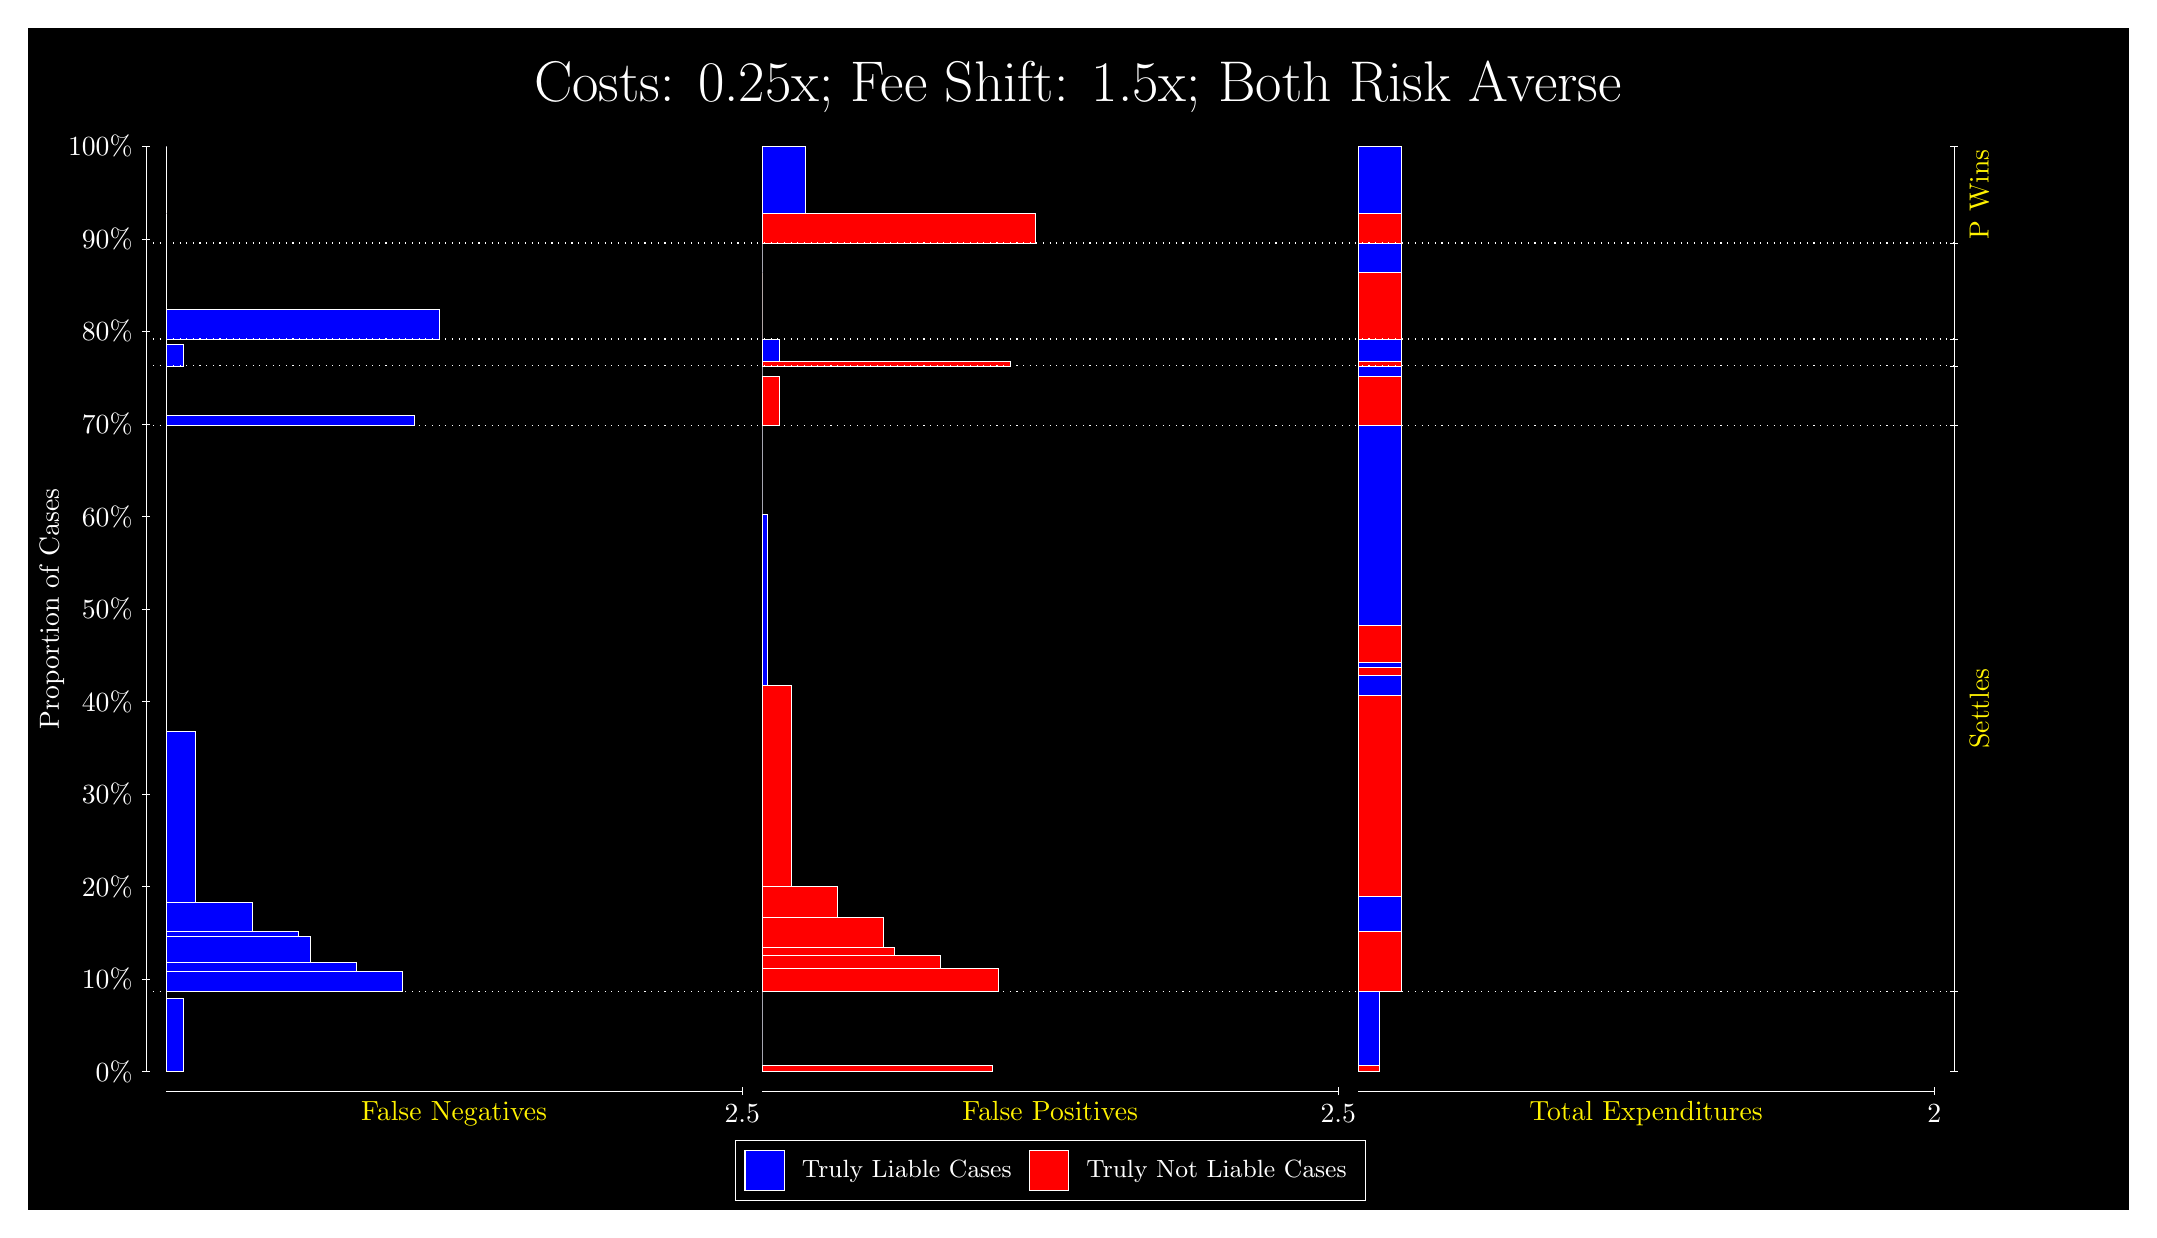
\begin{tikzpicture}
\draw[fill=black] (0,0) rectangle (26.667,15);
\draw[text=white] (0,13.5) rectangle (26.667,15) node[midway] {\huge Costs: 0.25x; Fee Shift: 1.5x; Both Risk Averse};
\draw[white, very thin] (1.5,1.75) -- (1.5,13.5);
\node[rotate=90, text=white, anchor=center] at (0.3, 7.625) {Proportion of Cases};
\draw[white, very thin] (1.45,1.75) -- (1.55,1.75);
\node[text=white, anchor=east] at (1.45, 1.75) {0\%};
\draw[white, very thin] (1.45,2.925) -- (1.55,2.925);
\node[text=white, anchor=east] at (1.45, 2.925) {10\%};
\draw[white, very thin] (1.45,4.1) -- (1.55,4.1);
\node[text=white, anchor=east] at (1.45, 4.1) {20\%};
\draw[white, very thin] (1.45,5.275) -- (1.55,5.275);
\node[text=white, anchor=east] at (1.45, 5.275) {30\%};
\draw[white, very thin] (1.45,6.45) -- (1.55,6.45);
\node[text=white, anchor=east] at (1.45, 6.45) {40\%};
\draw[white, very thin] (1.45,7.625) -- (1.55,7.625);
\node[text=white, anchor=east] at (1.45, 7.625) {50\%};
\draw[white, very thin] (1.45,8.8) -- (1.55,8.8);
\node[text=white, anchor=east] at (1.45, 8.8) {60\%};
\draw[white, very thin] (1.45,9.975) -- (1.55,9.975);
\node[text=white, anchor=east] at (1.45, 9.975) {70\%};
\draw[white, very thin] (1.45,11.15) -- (1.55,11.15);
\node[text=white, anchor=east] at (1.45, 11.15) {80\%};
\draw[white, very thin] (1.45,12.325) -- (1.55,12.325);
\node[text=white, anchor=east] at (1.45, 12.325) {90\%};
\draw[white, very thin] (1.45,13.5) -- (1.55,13.5);
\node[text=white, anchor=east] at (1.45, 13.5) {100\%};

\draw[white, very thin] (24.457,1.75) -- (24.457,13.5);
\draw[white, very thin] (24.407,1.75) -- (24.507,1.75);
\node[anchor=west] at (24.407, 1.75) {};
\draw[white, very thin] (24.407,2.7635) -- (24.507,2.7635);
\node[anchor=west] at (24.407, 2.7635) {};
\draw[white, very thin] (24.407,9.9567) -- (24.507,9.9567);
\node[anchor=west] at (24.407, 9.9567) {};
\draw[white, very thin] (24.407,10.712) -- (24.507,10.712);
\node[anchor=west] at (24.407, 10.712) {};
\draw[white, very thin] (24.407,11.053) -- (24.507,11.053);
\node[anchor=west] at (24.407, 11.053) {};
\draw[white, very thin] (24.407,12.272) -- (24.507,12.272);
\node[anchor=west] at (24.407, 12.272) {};
\draw[white, very thin] (24.407,13.5) -- (24.507,13.5);
\node[anchor=west] at (24.407, 13.5) {};

\draw[white, very thin, fill=blue] (1.75,1.75) rectangle (1.9696,2.6814);
\draw[white, very thin, fill=red] (1.75,2.6814) rectangle (1.75,2.7635);
\draw[white, very thin, fill=blue] (1.75,2.7635) rectangle (4.7507,3.0211);
\draw[white, very thin, fill=blue] (1.75,3.0211) rectangle (4.1652,3.1397);
\draw[white, very thin, fill=blue] (1.75,3.1397) rectangle (3.5797,3.4651);
\draw[white, very thin, fill=blue] (1.75,3.4651) rectangle (3.4333,3.5351);
\draw[white, very thin, fill=blue] (1.75,3.5351) rectangle (2.8478,3.8962);
\draw[white, very thin, fill=blue] (1.75,3.8962) rectangle (2.1159,6.0701);
\draw[white, very thin, fill=red] (1.75,6.0701) rectangle (1.75,9.9567);
\draw[white, very thin, fill=blue] (1.75,9.9567) rectangle (4.8971,10.085);
\draw[white, very thin, fill=red] (1.75,10.085) rectangle (1.75,10.712);
\draw[white, very thin, fill=blue] (1.75,10.712) rectangle (1.9696,10.992);
\draw[white, very thin, fill=red] (1.75,10.992) rectangle (1.75,11.053);
\draw[white, very thin, fill=blue] (1.75,11.053) rectangle (5.2265,11.429);
\draw[white, very thin, fill=red] (1.75,11.429) rectangle (1.75,12.272);
\draw[white, very thin, fill=red] (1.75,12.272) rectangle (1.75,12.648);
\draw[white, very thin, fill=blue] (1.75,12.648) rectangle (1.75,13.5);
\draw[white, very thin, fill=red] (9.3189,1.75) rectangle (12.246,1.832);
\draw[white, very thin, fill=blue] (9.3189,1.832) rectangle (9.3189,2.7635);
\draw[white, very thin, fill=red] (9.3189,2.7635) rectangle (12.32,3.0614);
\draw[white, very thin, fill=red] (9.3189,3.0614) rectangle (11.588,3.2325);
\draw[white, very thin, fill=red] (9.3189,3.2325) rectangle (11.002,3.3279);
\draw[white, very thin, fill=red] (9.3189,3.3279) rectangle (10.856,3.7075);
\draw[white, very thin, fill=red] (9.3189,3.7075) rectangle (10.27,4.0993);
\draw[white, very thin, fill=red] (9.3189,4.0993) rectangle (9.6848,6.6501);
\draw[white, very thin, fill=blue] (9.3189,6.6501) rectangle (9.3921,8.824);
\draw[white, very thin, fill=blue] (9.3189,8.824) rectangle (9.3189,9.9567);
\draw[white, very thin, fill=red] (9.3189,9.9567) rectangle (9.5384,10.584);
\draw[white, very thin, fill=blue] (9.3189,10.584) rectangle (9.3189,10.712);
\draw[white, very thin, fill=red] (9.3189,10.712) rectangle (12.466,10.772);
\draw[white, very thin, fill=blue] (9.3189,10.772) rectangle (9.5384,11.053);
\draw[white, very thin, fill=red] (9.3189,11.053) rectangle (9.3189,11.895);
\draw[white, very thin, fill=blue] (9.3189,11.895) rectangle (9.3189,12.272);
\draw[white, very thin, fill=red] (9.3189,12.272) rectangle (12.795,12.648);
\draw[white, very thin, fill=blue] (9.3189,12.648) rectangle (9.8678,13.5);
\draw[white, very thin, fill=red] (16.888,1.75) rectangle (17.162,1.832);
\draw[white, very thin, fill=blue] (16.888,1.832) rectangle (17.162,2.7635);
\draw[white, very thin, fill=red] (16.888,2.7635) rectangle (17.437,3.5349);
\draw[white, very thin, fill=blue] (16.888,3.5349) rectangle (17.437,3.9788);
\draw[white, very thin, fill=red] (16.888,3.9788) rectangle (17.437,6.5296);
\draw[white, very thin, fill=blue] (16.888,6.5296) rectangle (17.437,6.7872);
\draw[white, very thin, fill=red] (16.888,6.7872) rectangle (17.437,6.8827);
\draw[white, very thin, fill=blue] (16.888,6.8827) rectangle (17.437,6.9527);
\draw[white, very thin, fill=red] (16.888,6.9527) rectangle (17.437,7.4217);
\draw[white, very thin, fill=blue] (16.888,7.4217) rectangle (17.437,9.9567);
\draw[white, very thin, fill=red] (16.888,9.9567) rectangle (17.437,10.584);
\draw[white, very thin, fill=blue] (16.888,10.584) rectangle (17.437,10.712);
\draw[white, very thin, fill=red] (16.888,10.712) rectangle (17.437,10.772);
\draw[white, very thin, fill=blue] (16.888,10.772) rectangle (17.437,11.053);
\draw[white, very thin, fill=red] (16.888,11.053) rectangle (17.437,11.895);
\draw[white, very thin, fill=blue] (16.888,11.895) rectangle (17.437,12.272);
\draw[white, very thin, fill=red] (16.888,12.272) rectangle (17.437,12.648);
\draw[white, very thin, fill=blue] (16.888,12.648) rectangle (17.437,13.5);
\draw[white, dotted] (1.5,2.7635) -- (24.457,2.7635);
\draw[white, dotted] (1.5,9.9567) -- (24.457,9.9567);
\draw[white, dotted] (1.5,10.712) -- (24.457,10.712);
\draw[white, dotted] (1.5,11.053) -- (24.457,11.053);
\draw[white, dotted] (1.5,12.272) -- (24.457,12.272);
\draw[white, very thin] (1.75,1.5) -- (9.0689,1.5);
\node[text=yellow, anchor=north] at (5.4094, 1.5) {False Negatives};
\draw[white, very thin] (9.0689,1.45) -- (9.0689,1.55);
\node[text=white, anchor=north] at (9.0689, 1.45) {2.5};

\draw[white, very thin] (9.3189,1.5) -- (16.638,1.5);
\node[text=yellow, anchor=north] at (12.978, 1.5) {False Positives};
\draw[white, very thin] (16.638,1.45) -- (16.638,1.55);
\node[text=white, anchor=north] at (16.638, 1.45) {2.5};

\draw[white, very thin] (16.888,1.5) -- (24.207,1.5);
\node[text=yellow, anchor=north] at (20.547, 1.5) {Total Expenditures};
\draw[white, very thin] (24.207,1.45) -- (24.207,1.55);
\node[text=white, anchor=north] at (24.207, 1.45) {2};


\node[text=yellow, centered, rotate=90] at (24.777, 6.3601) {Settles};



\node[text=yellow, centered, rotate=90] at (24.777, 12.886) {P Wins};

\draw (12.978300999999998,1.5) node[draw=none] (baseCoordinate) {};
\begin{scope}[align=center]
        \matrix[scale=0.5, draw=white, below=0.5cm of baseCoordinate, nodes={draw}, column sep=0.1cm]{
            \node[rectangle, draw, minimum width=0.5cm, minimum height=0.5cm, fill=blue] {}; &
            \node[draw=none, font=\small, text=white] (B) {Truly Liable Cases}; &
            \node[rectangle, draw, minimum width=0.5cm, minimum height=0.5cm, fill=red] {}; &
            \node[draw=none, font=\small, text=white] (B) {Truly Not Liable Cases}; \\
            };
\end{scope}

\end{tikzpicture}
\end{document}